% c3_address.tex — C³ Address System and Unit Interface
% Fragment file: % c3_address.tex — C³ Address System and Unit Interface
% Fragment file: % c3_address.tex — C³ Address System and Unit Interface
% Fragment file: % c3_address.tex — C³ Address System and Unit Interface
% Fragment file: \input{sections/c3_address} from main document
% Requires: tikz, booktabs, array, xcolor

%% ============================================================
%%  SECTION 1 — Universal Spectral Address System
%% ============================================================
\section{Universal Spectral Address System}
\label{sec:spectral-address}

Every datum flowing through the MI pipeline carries a \emph{spectral address}:
a four-component tuple that uniquely identifies its origin in the
R\textsuperscript{3}--H\textsuperscript{3} feature--temporal lattice.

\medskip

\begin{center}
\texttt{\{r3\_idx\}.\{horizon\}.\{morph\}.\{law\}}
\end{center}

\medskip

\noindent
\textbf{Numeric example:}\quad \texttt{83.H12.M9.L0}\\[2pt]
\textbf{Spectral label:}\quad
\texttt{chroma\_frame\_distance.beat.velocity\_mean.memory}

% ---- TikZ address decomposition diagram ----
\begin{figure}[ht]
\centering
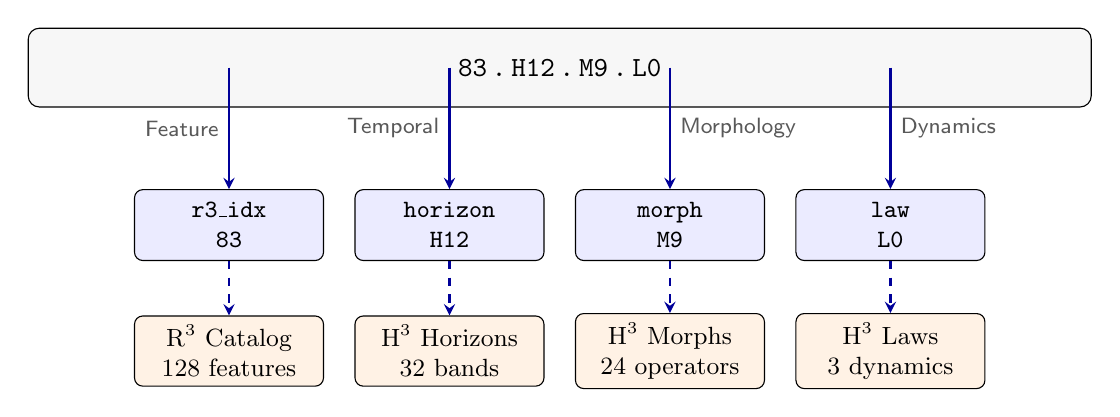
\begin{tikzpicture}[
    comp/.style={
        draw, rounded corners=3pt, fill=blue!8,
        minimum width=2.4cm, minimum height=0.9cm,
        font=\small\ttfamily, align=center
    },
    catalog/.style={
        draw, rounded corners=3pt, fill=orange!10,
        minimum width=2.4cm, minimum height=0.7cm,
        font=\small, align=center
    },
    arr/.style={->, >=stealth, thick, color=blue!60!black},
    lbl/.style={font=\footnotesize\sffamily, color=gray!70!black}
]
    % Full address bar
    \node[draw, rounded corners=4pt, fill=gray!6,
          minimum width=13.5cm, minimum height=1.0cm,
          font=\ttfamily]
        (addr) at (0,0) {83\,.\,H12\,.\,M9\,.\,L0};

    % Invisible anchors for the four segments
    \coordinate (a1) at (-4.2, 0);
    \coordinate (a2) at (-1.4, 0);
    \coordinate (a3) at ( 1.4, 0);
    \coordinate (a4) at ( 4.2, 0);

    % Component boxes below
    \node[comp] (c1) at (-4.2,-2.0) {r3\_idx\\83};
    \node[comp] (c2) at (-1.4,-2.0) {horizon\\H12};
    \node[comp] (c3) at ( 1.4,-2.0) {morph\\M9};
    \node[comp] (c4) at ( 4.2,-2.0) {law\\L0};

    % Arrows from address bar to components
    \draw[arr] (a1) -- (c1) node[midway, left, lbl] {Feature};
    \draw[arr] (a2) -- (c2) node[midway, left, lbl] {Temporal};
    \draw[arr] (a3) -- (c3) node[midway, right, lbl] {Morphology};
    \draw[arr] (a4) -- (c4) node[midway, right, lbl] {Dynamics};

    % Catalog / source layer below components
    \node[catalog] (s1) at (-4.2,-3.6) {R\textsuperscript{3} Catalog\\128 features};
    \node[catalog] (s2) at (-1.4,-3.6) {H\textsuperscript{3} Horizons\\32 bands};
    \node[catalog] (s3) at ( 1.4,-3.6) {H\textsuperscript{3} Morphs\\24 operators};
    \node[catalog] (s4) at ( 4.2,-3.6) {H\textsuperscript{3} Laws\\3 dynamics};

    \draw[arr, dashed] (c1) -- (s1);
    \draw[arr, dashed] (c2) -- (s2);
    \draw[arr, dashed] (c3) -- (s3);
    \draw[arr, dashed] (c4) -- (s4);
\end{tikzpicture}
\caption{Four-tuple spectral address decomposition.
         Each component maps to a specific catalog layer in the
         R\textsuperscript{3}/H\textsuperscript{3} system.}
\label{fig:address-decomposition}
\end{figure}


% ---- Address Construction Rules table ----
\subsection{Address Construction Rules}
\label{subsec:address-rules}

\begin{table}[ht]
\centering
\caption{Address component construction rules.}
\label{tab:address-construction}
\begin{tabular}{@{}llll@{}}
\toprule
\textbf{Component} & \textbf{Source} & \textbf{Range} & \textbf{Example} \\
\midrule
\texttt{r3\_idx} & R\textsuperscript{3} Feature Index & 0--127  & 83  \\
\texttt{horizon} & H\textsuperscript{3} Horizon Index  & H0--H31 & H12 \\
\texttt{morph}   & H\textsuperscript{3} Morph Index    & M0--M23 & M9  \\
\texttt{law}     & H\textsuperscript{3} Law Index      & L0--L2  & L0  \\
\bottomrule
\end{tabular}
\end{table}


% ---- Spectral Label Construction table ----
\subsection{Spectral Label Construction}
\label{subsec:spectral-label}

\begin{table}[ht]
\centering
\caption{Spectral label construction from address components.}
\label{tab:spectral-label}
\begin{tabular}{@{}lll@{}}
\toprule
\textbf{Component} & \textbf{Format} & \textbf{Example} \\
\midrule
Feature    & R\textsuperscript{3} USL name   & \texttt{chroma\_frame\_distance} \\
Horizon    & H\textsuperscript{3} USL label  & \texttt{beat}                   \\
Morph      & H\textsuperscript{3} morph name & \texttt{velocity\_mean}         \\
Law        & H\textsuperscript{3} law name   & \texttt{memory}                 \\
\midrule
Full label & \texttt{feature.horizon.morph.law}
           & \texttt{chroma\_frame\_distance.beat.velocity\_mean.memory} \\
\bottomrule
\end{tabular}
\end{table}


%% ============================================================
%%  SECTION 2 — C³ Unit Interface Table
%% ============================================================
\section{C\textsuperscript{3} Unit Interface Table}
\label{sec:c3-units}

Table~\ref{tab:c3-units} lists all nine C\textsuperscript{3} processing units
and their primary interfaces with the R\textsuperscript{3} feature groups and
H\textsuperscript{3} temporal bands.
R\textsuperscript{3} groups are identified by letter
(A~=~Consonance, B~=~Energy, C~=~Timbre, D~=~Change, E~=~Interactions,
 F~=~Pitch-Class, G~=~Onset Period, H~=~Harmony, I~=~Information,
 J~=~Timbre Ext., K~=~Modulation).
H\textsuperscript{3} bands span Micro ($<$50\,ms), Meso (50\,ms--2\,s),
and Macro ($>$2\,s) perceptual time scales.

\begin{table}[ht]
\centering
\caption{C\textsuperscript{3} unit interface summary.}
\label{tab:c3-units}
\renewcommand{\arraystretch}{1.15}
\begin{tabular}{@{}llclll@{}}
\toprule
\textbf{Unit} & \textbf{Full Name}
  & \textbf{Models}
  & \textbf{Primary R\textsuperscript{3} Groups}
  & \textbf{Primary H\textsuperscript{3} Bands}
  & \textbf{Primary Laws} \\
\midrule
SPU & Sensory Processing    &  9 & A, B, C, D & Micro--Meso  & L0, L2        \\
STU & Structural Timing     & 20 & G, H, I    & Meso--Macro  & L0, L1, L2    \\
IMU & Integrative Memory    & 10 & F, H, I    & Meso--Macro  & L0, L2        \\
ASU & Auditory Scene        &  9 & A, B, C    & Micro--Meso  & L2            \\
NDU & Neuromodulation       &  8 & B, H, I    & Meso--Macro  & L0, L1, L2    \\
MPU & Motor Planning        & 11 & G, H       & Meso         & L0, L1        \\
PCU & Predictive Coding     & 10 & F, H, I    & Micro--Macro & L0, L1, L2    \\
ARU & Arousal Regulation    &  9 & B, H, I    & Meso--Macro  & L0, L1, L2    \\
RPU & Reward Processing     & 10 & H, I, K    & Meso--Macro  & L0, L1, L2    \\
\bottomrule
\end{tabular}
\end{table}


%% ============================================================
%%  SECTION 3 — Provenance Chain Diagram
%% ============================================================
\section{Provenance Chain}
\label{sec:provenance-chain}

Figure~\ref{fig:provenance} traces the complete data-flow from raw audio
to the C\textsuperscript{3} input package.  Every tensor element retains a
spectral address linking it back to its R\textsuperscript{3} source through
an unbroken provenance chain.

\begin{figure}[ht]
\centering
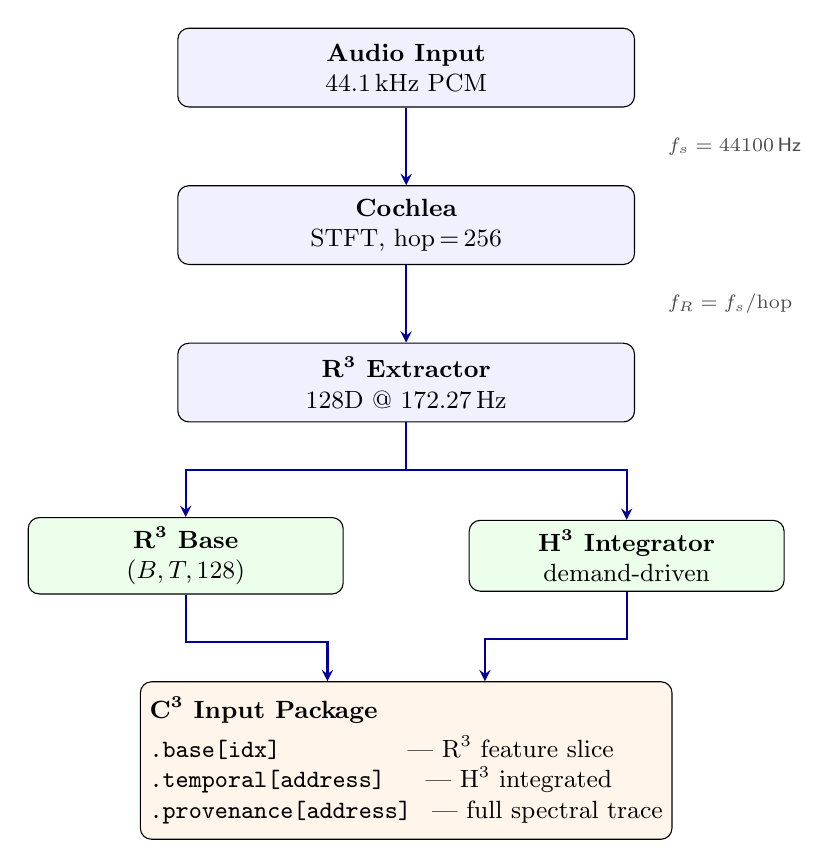
\begin{tikzpicture}[
    block/.style={
        draw, rounded corners=4pt, fill=blue!6,
        minimum width=5.8cm, minimum height=1.0cm,
        font=\small, align=center
    },
    split/.style={
        draw, rounded corners=4pt, fill=green!8,
        minimum width=4.0cm, minimum height=0.9cm,
        font=\small, align=center
    },
    pkg/.style={
        draw, rounded corners=4pt, fill=orange!8,
        minimum width=6.4cm, minimum height=2.0cm,
        font=\small, align=left
    },
    arr/.style={->, >=stealth, thick, color=blue!60!black},
    note/.style={font=\scriptsize\sffamily, color=gray!60!black}
]
    % Top: Audio input
    \node[block] (audio) at (0, 0)
        {\textbf{Audio Input}\\44.1\,kHz PCM};

    % Cochlea
    \node[block] (cochlea) at (0, -2.0)
        {\textbf{Cochlea}\\STFT, hop\,=\,256};
    \draw[arr] (audio) -- (cochlea);
    \node[note, right] at (3.2, -1.0) {$f_s = 44100$\,Hz};

    % R³ Extractor
    \node[block] (r3ext) at (0, -4.0)
        {\textbf{R\textsuperscript{3} Extractor}\\128D @ 172.27\,Hz};
    \draw[arr] (cochlea) -- (r3ext);
    \node[note, right] at (3.2, -3.0) {$f_R = f_s / \mathrm{hop}$};

    % Split into two branches
    \node[split] (r3base) at (-2.8, -6.2)
        {\textbf{R\textsuperscript{3} Base}\\$(B, T, 128)$};
    \node[split] (h3int)  at ( 2.8, -6.2)
        {\textbf{H\textsuperscript{3} Integrator}\\demand-driven};

    \draw[arr] (r3ext.south) -- ++(0,-0.6) -| (r3base.north);
    \draw[arr] (r3ext.south) -- ++(0,-0.6) -| (h3int.north);

    % C³ Input Package
    \node[pkg] (c3pkg) at (0, -8.8)
        {\textbf{C\textsuperscript{3} Input Package}\\[3pt]
         \texttt{.base[idx]}
         \hspace{1.4cm} \textrm{--- R\textsuperscript{3} feature slice}\\
         \texttt{.temporal[address]}
         \hspace{0.3cm} \textrm{--- H\textsuperscript{3} integrated}\\
         \texttt{.provenance[address]}
         \hspace{0.05cm} \textrm{--- full spectral trace}};

    \draw[arr] (r3base.south)  -- ++(0,-0.6) -| ([xshift=-1cm]c3pkg.north);
    \draw[arr] (h3int.south)   -- ++(0,-0.6) -| ([xshift= 1cm]c3pkg.north);
\end{tikzpicture}
\caption{Provenance chain from audio input to C\textsuperscript{3} input package.
         Every tensor element traces back to its R\textsuperscript{3} source
         through spectral addresses.}
\label{fig:provenance}
\end{figure}


%% ============================================================
%%  SECTION 4 — Naming Convention Rules
%% ============================================================
\section{Naming Convention Rules}
\label{sec:naming-rules}

The following rules govern all naming within the Universal Spectral Language.
Violations break the provenance chain and are treated as specification errors.

\begin{enumerate}
    \item \textbf{Measurement, not interpretation.}\enspace
          R\textsuperscript{3} feature names describe what is \emph{measured}
          (e.g.\ \texttt{spectral\_centroid}), never what is
          \emph{perceived} or \emph{interpreted}.

    \item \textbf{No music-theory terms in R\textsuperscript{3}/H\textsuperscript{3}.}\enspace
          Names must not contain \texttt{chord}, \texttt{key},
          \texttt{cadence}, \texttt{tonal}, or \texttt{harmonic}
          in their music-theoretic senses.
          \texttt{harmonic} is permitted only in its signal-processing
          meaning (integer-multiple partials).

    \item \textbf{Perceptual time scales, not musical structure.}\enspace
          H\textsuperscript{3} horizon labels denote perceptual durations.
          For example, \texttt{beat} designates the ${\sim}525$\,ms
          periodicity band, not a musical beat or metrical position.

    \item \textbf{Dot-separated addresses.}\enspace
          Full spectral addresses use dot separation:
          \texttt{feature.horizon.morph.law}.
          No spaces, no slashes, no camelCase.

    \item \textbf{C\textsuperscript{3} music-theory mapping.}\enspace
          C\textsuperscript{3} model documentation \emph{may} reference
          music-theory terms for explanatory purposes, but every such
          reference \emph{must} map to one or more spectral addresses.

    \item \textbf{Unbroken spectral chain.}\enspace
          Every C\textsuperscript{3} input must trace back to an
          R\textsuperscript{3} source through the address system.
          No datum enters C\textsuperscript{3} without a provenance record.
\end{enumerate}
 from main document
% Requires: tikz, booktabs, array, xcolor

%% ============================================================
%%  SECTION 1 — Universal Spectral Address System
%% ============================================================
\section{Universal Spectral Address System}
\label{sec:spectral-address}

Every datum flowing through the MI pipeline carries a \emph{spectral address}:
a four-component tuple that uniquely identifies its origin in the
R\textsuperscript{3}--H\textsuperscript{3} feature--temporal lattice.

\medskip

\begin{center}
\texttt{\{r3\_idx\}.\{horizon\}.\{morph\}.\{law\}}
\end{center}

\medskip

\noindent
\textbf{Numeric example:}\quad \texttt{83.H12.M9.L0}\\[2pt]
\textbf{Spectral label:}\quad
\texttt{chroma\_frame\_distance.beat.velocity\_mean.memory}

% ---- TikZ address decomposition diagram ----
\begin{figure}[ht]
\centering
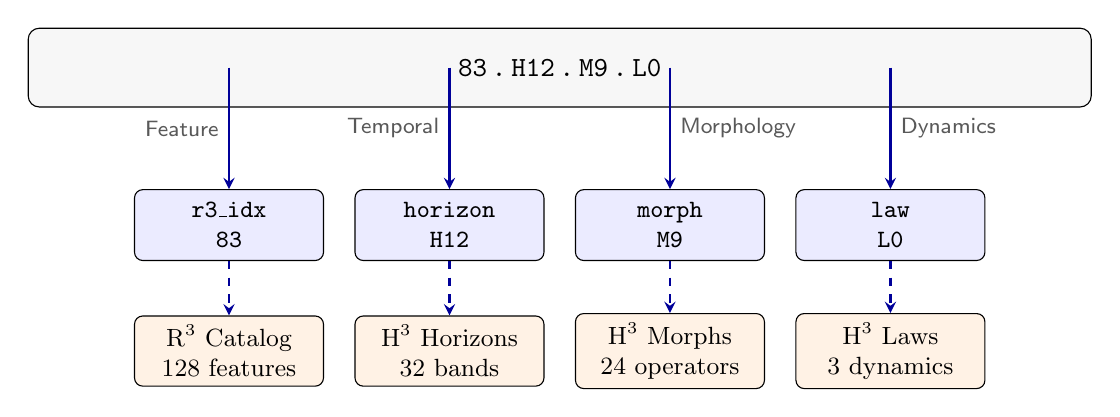
\begin{tikzpicture}[
    comp/.style={
        draw, rounded corners=3pt, fill=blue!8,
        minimum width=2.4cm, minimum height=0.9cm,
        font=\small\ttfamily, align=center
    },
    catalog/.style={
        draw, rounded corners=3pt, fill=orange!10,
        minimum width=2.4cm, minimum height=0.7cm,
        font=\small, align=center
    },
    arr/.style={->, >=stealth, thick, color=blue!60!black},
    lbl/.style={font=\footnotesize\sffamily, color=gray!70!black}
]
    % Full address bar
    \node[draw, rounded corners=4pt, fill=gray!6,
          minimum width=13.5cm, minimum height=1.0cm,
          font=\ttfamily]
        (addr) at (0,0) {83\,.\,H12\,.\,M9\,.\,L0};

    % Invisible anchors for the four segments
    \coordinate (a1) at (-4.2, 0);
    \coordinate (a2) at (-1.4, 0);
    \coordinate (a3) at ( 1.4, 0);
    \coordinate (a4) at ( 4.2, 0);

    % Component boxes below
    \node[comp] (c1) at (-4.2,-2.0) {r3\_idx\\83};
    \node[comp] (c2) at (-1.4,-2.0) {horizon\\H12};
    \node[comp] (c3) at ( 1.4,-2.0) {morph\\M9};
    \node[comp] (c4) at ( 4.2,-2.0) {law\\L0};

    % Arrows from address bar to components
    \draw[arr] (a1) -- (c1) node[midway, left, lbl] {Feature};
    \draw[arr] (a2) -- (c2) node[midway, left, lbl] {Temporal};
    \draw[arr] (a3) -- (c3) node[midway, right, lbl] {Morphology};
    \draw[arr] (a4) -- (c4) node[midway, right, lbl] {Dynamics};

    % Catalog / source layer below components
    \node[catalog] (s1) at (-4.2,-3.6) {R\textsuperscript{3} Catalog\\128 features};
    \node[catalog] (s2) at (-1.4,-3.6) {H\textsuperscript{3} Horizons\\32 bands};
    \node[catalog] (s3) at ( 1.4,-3.6) {H\textsuperscript{3} Morphs\\24 operators};
    \node[catalog] (s4) at ( 4.2,-3.6) {H\textsuperscript{3} Laws\\3 dynamics};

    \draw[arr, dashed] (c1) -- (s1);
    \draw[arr, dashed] (c2) -- (s2);
    \draw[arr, dashed] (c3) -- (s3);
    \draw[arr, dashed] (c4) -- (s4);
\end{tikzpicture}
\caption{Four-tuple spectral address decomposition.
         Each component maps to a specific catalog layer in the
         R\textsuperscript{3}/H\textsuperscript{3} system.}
\label{fig:address-decomposition}
\end{figure}


% ---- Address Construction Rules table ----
\subsection{Address Construction Rules}
\label{subsec:address-rules}

\begin{table}[ht]
\centering
\caption{Address component construction rules.}
\label{tab:address-construction}
\begin{tabular}{@{}llll@{}}
\toprule
\textbf{Component} & \textbf{Source} & \textbf{Range} & \textbf{Example} \\
\midrule
\texttt{r3\_idx} & R\textsuperscript{3} Feature Index & 0--127  & 83  \\
\texttt{horizon} & H\textsuperscript{3} Horizon Index  & H0--H31 & H12 \\
\texttt{morph}   & H\textsuperscript{3} Morph Index    & M0--M23 & M9  \\
\texttt{law}     & H\textsuperscript{3} Law Index      & L0--L2  & L0  \\
\bottomrule
\end{tabular}
\end{table}


% ---- Spectral Label Construction table ----
\subsection{Spectral Label Construction}
\label{subsec:spectral-label}

\begin{table}[ht]
\centering
\caption{Spectral label construction from address components.}
\label{tab:spectral-label}
\begin{tabular}{@{}lll@{}}
\toprule
\textbf{Component} & \textbf{Format} & \textbf{Example} \\
\midrule
Feature    & R\textsuperscript{3} USL name   & \texttt{chroma\_frame\_distance} \\
Horizon    & H\textsuperscript{3} USL label  & \texttt{beat}                   \\
Morph      & H\textsuperscript{3} morph name & \texttt{velocity\_mean}         \\
Law        & H\textsuperscript{3} law name   & \texttt{memory}                 \\
\midrule
Full label & \texttt{feature.horizon.morph.law}
           & \texttt{chroma\_frame\_distance.beat.velocity\_mean.memory} \\
\bottomrule
\end{tabular}
\end{table}


%% ============================================================
%%  SECTION 2 — C³ Unit Interface Table
%% ============================================================
\section{C\textsuperscript{3} Unit Interface Table}
\label{sec:c3-units}

Table~\ref{tab:c3-units} lists all nine C\textsuperscript{3} processing units
and their primary interfaces with the R\textsuperscript{3} feature groups and
H\textsuperscript{3} temporal bands.
R\textsuperscript{3} groups are identified by letter
(A~=~Consonance, B~=~Energy, C~=~Timbre, D~=~Change, E~=~Interactions,
 F~=~Pitch-Class, G~=~Onset Period, H~=~Harmony, I~=~Information,
 J~=~Timbre Ext., K~=~Modulation).
H\textsuperscript{3} bands span Micro ($<$50\,ms), Meso (50\,ms--2\,s),
and Macro ($>$2\,s) perceptual time scales.

\begin{table}[ht]
\centering
\caption{C\textsuperscript{3} unit interface summary.}
\label{tab:c3-units}
\renewcommand{\arraystretch}{1.15}
\begin{tabular}{@{}llclll@{}}
\toprule
\textbf{Unit} & \textbf{Full Name}
  & \textbf{Models}
  & \textbf{Primary R\textsuperscript{3} Groups}
  & \textbf{Primary H\textsuperscript{3} Bands}
  & \textbf{Primary Laws} \\
\midrule
SPU & Sensory Processing    &  9 & A, B, C, D & Micro--Meso  & L0, L2        \\
STU & Structural Timing     & 20 & G, H, I    & Meso--Macro  & L0, L1, L2    \\
IMU & Integrative Memory    & 10 & F, H, I    & Meso--Macro  & L0, L2        \\
ASU & Auditory Scene        &  9 & A, B, C    & Micro--Meso  & L2            \\
NDU & Neuromodulation       &  8 & B, H, I    & Meso--Macro  & L0, L1, L2    \\
MPU & Motor Planning        & 11 & G, H       & Meso         & L0, L1        \\
PCU & Predictive Coding     & 10 & F, H, I    & Micro--Macro & L0, L1, L2    \\
ARU & Arousal Regulation    &  9 & B, H, I    & Meso--Macro  & L0, L1, L2    \\
RPU & Reward Processing     & 10 & H, I, K    & Meso--Macro  & L0, L1, L2    \\
\bottomrule
\end{tabular}
\end{table}


%% ============================================================
%%  SECTION 3 — Provenance Chain Diagram
%% ============================================================
\section{Provenance Chain}
\label{sec:provenance-chain}

Figure~\ref{fig:provenance} traces the complete data-flow from raw audio
to the C\textsuperscript{3} input package.  Every tensor element retains a
spectral address linking it back to its R\textsuperscript{3} source through
an unbroken provenance chain.

\begin{figure}[ht]
\centering
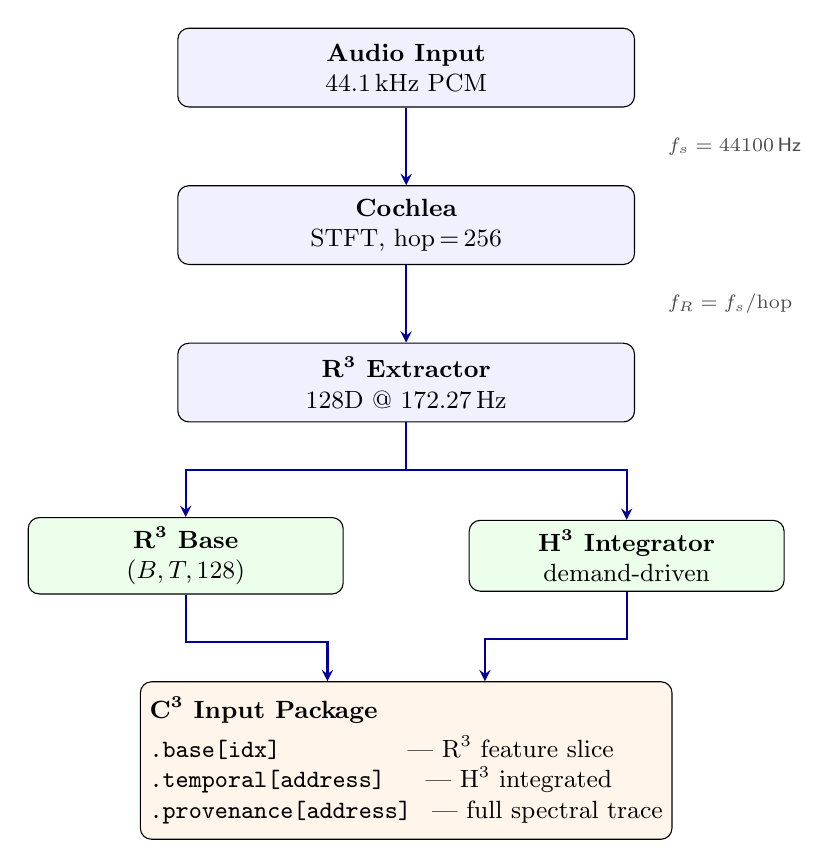
\begin{tikzpicture}[
    block/.style={
        draw, rounded corners=4pt, fill=blue!6,
        minimum width=5.8cm, minimum height=1.0cm,
        font=\small, align=center
    },
    split/.style={
        draw, rounded corners=4pt, fill=green!8,
        minimum width=4.0cm, minimum height=0.9cm,
        font=\small, align=center
    },
    pkg/.style={
        draw, rounded corners=4pt, fill=orange!8,
        minimum width=6.4cm, minimum height=2.0cm,
        font=\small, align=left
    },
    arr/.style={->, >=stealth, thick, color=blue!60!black},
    note/.style={font=\scriptsize\sffamily, color=gray!60!black}
]
    % Top: Audio input
    \node[block] (audio) at (0, 0)
        {\textbf{Audio Input}\\44.1\,kHz PCM};

    % Cochlea
    \node[block] (cochlea) at (0, -2.0)
        {\textbf{Cochlea}\\STFT, hop\,=\,256};
    \draw[arr] (audio) -- (cochlea);
    \node[note, right] at (3.2, -1.0) {$f_s = 44100$\,Hz};

    % R³ Extractor
    \node[block] (r3ext) at (0, -4.0)
        {\textbf{R\textsuperscript{3} Extractor}\\128D @ 172.27\,Hz};
    \draw[arr] (cochlea) -- (r3ext);
    \node[note, right] at (3.2, -3.0) {$f_R = f_s / \mathrm{hop}$};

    % Split into two branches
    \node[split] (r3base) at (-2.8, -6.2)
        {\textbf{R\textsuperscript{3} Base}\\$(B, T, 128)$};
    \node[split] (h3int)  at ( 2.8, -6.2)
        {\textbf{H\textsuperscript{3} Integrator}\\demand-driven};

    \draw[arr] (r3ext.south) -- ++(0,-0.6) -| (r3base.north);
    \draw[arr] (r3ext.south) -- ++(0,-0.6) -| (h3int.north);

    % C³ Input Package
    \node[pkg] (c3pkg) at (0, -8.8)
        {\textbf{C\textsuperscript{3} Input Package}\\[3pt]
         \texttt{.base[idx]}
         \hspace{1.4cm} \textrm{--- R\textsuperscript{3} feature slice}\\
         \texttt{.temporal[address]}
         \hspace{0.3cm} \textrm{--- H\textsuperscript{3} integrated}\\
         \texttt{.provenance[address]}
         \hspace{0.05cm} \textrm{--- full spectral trace}};

    \draw[arr] (r3base.south)  -- ++(0,-0.6) -| ([xshift=-1cm]c3pkg.north);
    \draw[arr] (h3int.south)   -- ++(0,-0.6) -| ([xshift= 1cm]c3pkg.north);
\end{tikzpicture}
\caption{Provenance chain from audio input to C\textsuperscript{3} input package.
         Every tensor element traces back to its R\textsuperscript{3} source
         through spectral addresses.}
\label{fig:provenance}
\end{figure}


%% ============================================================
%%  SECTION 4 — Naming Convention Rules
%% ============================================================
\section{Naming Convention Rules}
\label{sec:naming-rules}

The following rules govern all naming within the Universal Spectral Language.
Violations break the provenance chain and are treated as specification errors.

\begin{enumerate}
    \item \textbf{Measurement, not interpretation.}\enspace
          R\textsuperscript{3} feature names describe what is \emph{measured}
          (e.g.\ \texttt{spectral\_centroid}), never what is
          \emph{perceived} or \emph{interpreted}.

    \item \textbf{No music-theory terms in R\textsuperscript{3}/H\textsuperscript{3}.}\enspace
          Names must not contain \texttt{chord}, \texttt{key},
          \texttt{cadence}, \texttt{tonal}, or \texttt{harmonic}
          in their music-theoretic senses.
          \texttt{harmonic} is permitted only in its signal-processing
          meaning (integer-multiple partials).

    \item \textbf{Perceptual time scales, not musical structure.}\enspace
          H\textsuperscript{3} horizon labels denote perceptual durations.
          For example, \texttt{beat} designates the ${\sim}525$\,ms
          periodicity band, not a musical beat or metrical position.

    \item \textbf{Dot-separated addresses.}\enspace
          Full spectral addresses use dot separation:
          \texttt{feature.horizon.morph.law}.
          No spaces, no slashes, no camelCase.

    \item \textbf{C\textsuperscript{3} music-theory mapping.}\enspace
          C\textsuperscript{3} model documentation \emph{may} reference
          music-theory terms for explanatory purposes, but every such
          reference \emph{must} map to one or more spectral addresses.

    \item \textbf{Unbroken spectral chain.}\enspace
          Every C\textsuperscript{3} input must trace back to an
          R\textsuperscript{3} source through the address system.
          No datum enters C\textsuperscript{3} without a provenance record.
\end{enumerate}
 from main document
% Requires: tikz, booktabs, array, xcolor

%% ============================================================
%%  SECTION 1 — Universal Spectral Address System
%% ============================================================
\section{Universal Spectral Address System}
\label{sec:spectral-address}

Every datum flowing through the MI pipeline carries a \emph{spectral address}:
a four-component tuple that uniquely identifies its origin in the
R\textsuperscript{3}--H\textsuperscript{3} feature--temporal lattice.

\medskip

\begin{center}
\texttt{\{r3\_idx\}.\{horizon\}.\{morph\}.\{law\}}
\end{center}

\medskip

\noindent
\textbf{Numeric example:}\quad \texttt{83.H12.M9.L0}\\[2pt]
\textbf{Spectral label:}\quad
\texttt{chroma\_frame\_distance.beat.velocity\_mean.memory}

% ---- TikZ address decomposition diagram ----
\begin{figure}[ht]
\centering
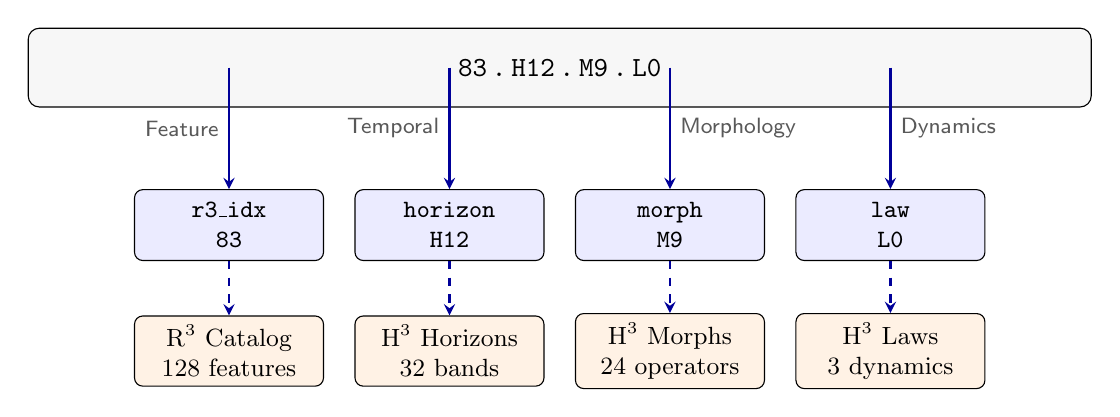
\begin{tikzpicture}[
    comp/.style={
        draw, rounded corners=3pt, fill=blue!8,
        minimum width=2.4cm, minimum height=0.9cm,
        font=\small\ttfamily, align=center
    },
    catalog/.style={
        draw, rounded corners=3pt, fill=orange!10,
        minimum width=2.4cm, minimum height=0.7cm,
        font=\small, align=center
    },
    arr/.style={->, >=stealth, thick, color=blue!60!black},
    lbl/.style={font=\footnotesize\sffamily, color=gray!70!black}
]
    % Full address bar
    \node[draw, rounded corners=4pt, fill=gray!6,
          minimum width=13.5cm, minimum height=1.0cm,
          font=\ttfamily]
        (addr) at (0,0) {83\,.\,H12\,.\,M9\,.\,L0};

    % Invisible anchors for the four segments
    \coordinate (a1) at (-4.2, 0);
    \coordinate (a2) at (-1.4, 0);
    \coordinate (a3) at ( 1.4, 0);
    \coordinate (a4) at ( 4.2, 0);

    % Component boxes below
    \node[comp] (c1) at (-4.2,-2.0) {r3\_idx\\83};
    \node[comp] (c2) at (-1.4,-2.0) {horizon\\H12};
    \node[comp] (c3) at ( 1.4,-2.0) {morph\\M9};
    \node[comp] (c4) at ( 4.2,-2.0) {law\\L0};

    % Arrows from address bar to components
    \draw[arr] (a1) -- (c1) node[midway, left, lbl] {Feature};
    \draw[arr] (a2) -- (c2) node[midway, left, lbl] {Temporal};
    \draw[arr] (a3) -- (c3) node[midway, right, lbl] {Morphology};
    \draw[arr] (a4) -- (c4) node[midway, right, lbl] {Dynamics};

    % Catalog / source layer below components
    \node[catalog] (s1) at (-4.2,-3.6) {R\textsuperscript{3} Catalog\\128 features};
    \node[catalog] (s2) at (-1.4,-3.6) {H\textsuperscript{3} Horizons\\32 bands};
    \node[catalog] (s3) at ( 1.4,-3.6) {H\textsuperscript{3} Morphs\\24 operators};
    \node[catalog] (s4) at ( 4.2,-3.6) {H\textsuperscript{3} Laws\\3 dynamics};

    \draw[arr, dashed] (c1) -- (s1);
    \draw[arr, dashed] (c2) -- (s2);
    \draw[arr, dashed] (c3) -- (s3);
    \draw[arr, dashed] (c4) -- (s4);
\end{tikzpicture}
\caption{Four-tuple spectral address decomposition.
         Each component maps to a specific catalog layer in the
         R\textsuperscript{3}/H\textsuperscript{3} system.}
\label{fig:address-decomposition}
\end{figure}


% ---- Address Construction Rules table ----
\subsection{Address Construction Rules}
\label{subsec:address-rules}

\begin{table}[ht]
\centering
\caption{Address component construction rules.}
\label{tab:address-construction}
\begin{tabular}{@{}llll@{}}
\toprule
\textbf{Component} & \textbf{Source} & \textbf{Range} & \textbf{Example} \\
\midrule
\texttt{r3\_idx} & R\textsuperscript{3} Feature Index & 0--127  & 83  \\
\texttt{horizon} & H\textsuperscript{3} Horizon Index  & H0--H31 & H12 \\
\texttt{morph}   & H\textsuperscript{3} Morph Index    & M0--M23 & M9  \\
\texttt{law}     & H\textsuperscript{3} Law Index      & L0--L2  & L0  \\
\bottomrule
\end{tabular}
\end{table}


% ---- Spectral Label Construction table ----
\subsection{Spectral Label Construction}
\label{subsec:spectral-label}

\begin{table}[ht]
\centering
\caption{Spectral label construction from address components.}
\label{tab:spectral-label}
\begin{tabular}{@{}lll@{}}
\toprule
\textbf{Component} & \textbf{Format} & \textbf{Example} \\
\midrule
Feature    & R\textsuperscript{3} USL name   & \texttt{chroma\_frame\_distance} \\
Horizon    & H\textsuperscript{3} USL label  & \texttt{beat}                   \\
Morph      & H\textsuperscript{3} morph name & \texttt{velocity\_mean}         \\
Law        & H\textsuperscript{3} law name   & \texttt{memory}                 \\
\midrule
Full label & \texttt{feature.horizon.morph.law}
           & \texttt{chroma\_frame\_distance.beat.velocity\_mean.memory} \\
\bottomrule
\end{tabular}
\end{table}


%% ============================================================
%%  SECTION 2 — C³ Unit Interface Table
%% ============================================================
\section{C\textsuperscript{3} Unit Interface Table}
\label{sec:c3-units}

Table~\ref{tab:c3-units} lists all nine C\textsuperscript{3} processing units
and their primary interfaces with the R\textsuperscript{3} feature groups and
H\textsuperscript{3} temporal bands.
R\textsuperscript{3} groups are identified by letter
(A~=~Consonance, B~=~Energy, C~=~Timbre, D~=~Change, E~=~Interactions,
 F~=~Pitch-Class, G~=~Onset Period, H~=~Harmony, I~=~Information,
 J~=~Timbre Ext., K~=~Modulation).
H\textsuperscript{3} bands span Micro ($<$50\,ms), Meso (50\,ms--2\,s),
and Macro ($>$2\,s) perceptual time scales.

\begin{table}[ht]
\centering
\caption{C\textsuperscript{3} unit interface summary.}
\label{tab:c3-units}
\renewcommand{\arraystretch}{1.15}
\begin{tabular}{@{}llclll@{}}
\toprule
\textbf{Unit} & \textbf{Full Name}
  & \textbf{Models}
  & \textbf{Primary R\textsuperscript{3} Groups}
  & \textbf{Primary H\textsuperscript{3} Bands}
  & \textbf{Primary Laws} \\
\midrule
SPU & Sensory Processing    &  9 & A, B, C, D & Micro--Meso  & L0, L2        \\
STU & Structural Timing     & 20 & G, H, I    & Meso--Macro  & L0, L1, L2    \\
IMU & Integrative Memory    & 10 & F, H, I    & Meso--Macro  & L0, L2        \\
ASU & Auditory Scene        &  9 & A, B, C    & Micro--Meso  & L2            \\
NDU & Neuromodulation       &  8 & B, H, I    & Meso--Macro  & L0, L1, L2    \\
MPU & Motor Planning        & 11 & G, H       & Meso         & L0, L1        \\
PCU & Predictive Coding     & 10 & F, H, I    & Micro--Macro & L0, L1, L2    \\
ARU & Arousal Regulation    &  9 & B, H, I    & Meso--Macro  & L0, L1, L2    \\
RPU & Reward Processing     & 10 & H, I, K    & Meso--Macro  & L0, L1, L2    \\
\bottomrule
\end{tabular}
\end{table}


%% ============================================================
%%  SECTION 3 — Provenance Chain Diagram
%% ============================================================
\section{Provenance Chain}
\label{sec:provenance-chain}

Figure~\ref{fig:provenance} traces the complete data-flow from raw audio
to the C\textsuperscript{3} input package.  Every tensor element retains a
spectral address linking it back to its R\textsuperscript{3} source through
an unbroken provenance chain.

\begin{figure}[ht]
\centering
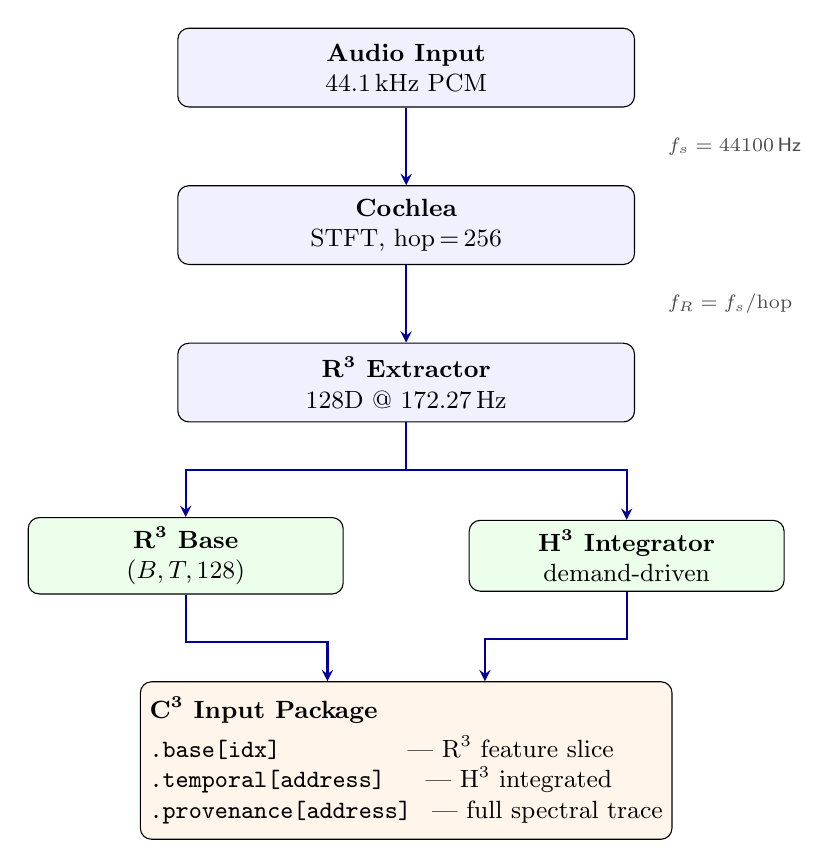
\begin{tikzpicture}[
    block/.style={
        draw, rounded corners=4pt, fill=blue!6,
        minimum width=5.8cm, minimum height=1.0cm,
        font=\small, align=center
    },
    split/.style={
        draw, rounded corners=4pt, fill=green!8,
        minimum width=4.0cm, minimum height=0.9cm,
        font=\small, align=center
    },
    pkg/.style={
        draw, rounded corners=4pt, fill=orange!8,
        minimum width=6.4cm, minimum height=2.0cm,
        font=\small, align=left
    },
    arr/.style={->, >=stealth, thick, color=blue!60!black},
    note/.style={font=\scriptsize\sffamily, color=gray!60!black}
]
    % Top: Audio input
    \node[block] (audio) at (0, 0)
        {\textbf{Audio Input}\\44.1\,kHz PCM};

    % Cochlea
    \node[block] (cochlea) at (0, -2.0)
        {\textbf{Cochlea}\\STFT, hop\,=\,256};
    \draw[arr] (audio) -- (cochlea);
    \node[note, right] at (3.2, -1.0) {$f_s = 44100$\,Hz};

    % R³ Extractor
    \node[block] (r3ext) at (0, -4.0)
        {\textbf{R\textsuperscript{3} Extractor}\\128D @ 172.27\,Hz};
    \draw[arr] (cochlea) -- (r3ext);
    \node[note, right] at (3.2, -3.0) {$f_R = f_s / \mathrm{hop}$};

    % Split into two branches
    \node[split] (r3base) at (-2.8, -6.2)
        {\textbf{R\textsuperscript{3} Base}\\$(B, T, 128)$};
    \node[split] (h3int)  at ( 2.8, -6.2)
        {\textbf{H\textsuperscript{3} Integrator}\\demand-driven};

    \draw[arr] (r3ext.south) -- ++(0,-0.6) -| (r3base.north);
    \draw[arr] (r3ext.south) -- ++(0,-0.6) -| (h3int.north);

    % C³ Input Package
    \node[pkg] (c3pkg) at (0, -8.8)
        {\textbf{C\textsuperscript{3} Input Package}\\[3pt]
         \texttt{.base[idx]}
         \hspace{1.4cm} \textrm{--- R\textsuperscript{3} feature slice}\\
         \texttt{.temporal[address]}
         \hspace{0.3cm} \textrm{--- H\textsuperscript{3} integrated}\\
         \texttt{.provenance[address]}
         \hspace{0.05cm} \textrm{--- full spectral trace}};

    \draw[arr] (r3base.south)  -- ++(0,-0.6) -| ([xshift=-1cm]c3pkg.north);
    \draw[arr] (h3int.south)   -- ++(0,-0.6) -| ([xshift= 1cm]c3pkg.north);
\end{tikzpicture}
\caption{Provenance chain from audio input to C\textsuperscript{3} input package.
         Every tensor element traces back to its R\textsuperscript{3} source
         through spectral addresses.}
\label{fig:provenance}
\end{figure}


%% ============================================================
%%  SECTION 4 — Naming Convention Rules
%% ============================================================
\section{Naming Convention Rules}
\label{sec:naming-rules}

The following rules govern all naming within the Universal Spectral Language.
Violations break the provenance chain and are treated as specification errors.

\begin{enumerate}
    \item \textbf{Measurement, not interpretation.}\enspace
          R\textsuperscript{3} feature names describe what is \emph{measured}
          (e.g.\ \texttt{spectral\_centroid}), never what is
          \emph{perceived} or \emph{interpreted}.

    \item \textbf{No music-theory terms in R\textsuperscript{3}/H\textsuperscript{3}.}\enspace
          Names must not contain \texttt{chord}, \texttt{key},
          \texttt{cadence}, \texttt{tonal}, or \texttt{harmonic}
          in their music-theoretic senses.
          \texttt{harmonic} is permitted only in its signal-processing
          meaning (integer-multiple partials).

    \item \textbf{Perceptual time scales, not musical structure.}\enspace
          H\textsuperscript{3} horizon labels denote perceptual durations.
          For example, \texttt{beat} designates the ${\sim}525$\,ms
          periodicity band, not a musical beat or metrical position.

    \item \textbf{Dot-separated addresses.}\enspace
          Full spectral addresses use dot separation:
          \texttt{feature.horizon.morph.law}.
          No spaces, no slashes, no camelCase.

    \item \textbf{C\textsuperscript{3} music-theory mapping.}\enspace
          C\textsuperscript{3} model documentation \emph{may} reference
          music-theory terms for explanatory purposes, but every such
          reference \emph{must} map to one or more spectral addresses.

    \item \textbf{Unbroken spectral chain.}\enspace
          Every C\textsuperscript{3} input must trace back to an
          R\textsuperscript{3} source through the address system.
          No datum enters C\textsuperscript{3} without a provenance record.
\end{enumerate}
 from main document
% Requires: tikz, booktabs, array, xcolor

%% ============================================================
%%  SECTION 1 — Universal Spectral Address System
%% ============================================================
\section{Universal Spectral Address System}
\label{sec:spectral-address}

Every datum flowing through the MI pipeline carries a \emph{spectral address}:
a four-component tuple that uniquely identifies its origin in the
R\textsuperscript{3}--H\textsuperscript{3} feature--temporal lattice.

\medskip

\begin{center}
\texttt{\{r3\_idx\}.\{horizon\}.\{morph\}.\{law\}}
\end{center}

\medskip

\noindent
\textbf{Numeric example:}\quad \texttt{83.H12.M9.L0}\\[2pt]
\textbf{Spectral label:}\quad
\texttt{chroma\_frame\_distance.beat.velocity\_mean.memory}

% ---- TikZ address decomposition diagram ----
\begin{figure}[ht]
\centering
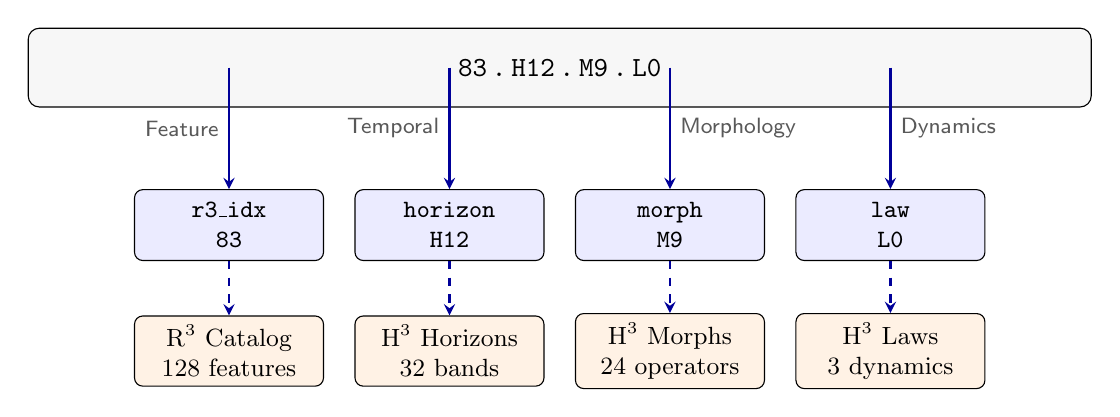
\begin{tikzpicture}[
    comp/.style={
        draw, rounded corners=3pt, fill=blue!8,
        minimum width=2.4cm, minimum height=0.9cm,
        font=\small\ttfamily, align=center
    },
    catalog/.style={
        draw, rounded corners=3pt, fill=orange!10,
        minimum width=2.4cm, minimum height=0.7cm,
        font=\small, align=center
    },
    arr/.style={->, >=stealth, thick, color=blue!60!black},
    lbl/.style={font=\footnotesize\sffamily, color=gray!70!black}
]
    % Full address bar
    \node[draw, rounded corners=4pt, fill=gray!6,
          minimum width=13.5cm, minimum height=1.0cm,
          font=\ttfamily]
        (addr) at (0,0) {83\,.\,H12\,.\,M9\,.\,L0};

    % Invisible anchors for the four segments
    \coordinate (a1) at (-4.2, 0);
    \coordinate (a2) at (-1.4, 0);
    \coordinate (a3) at ( 1.4, 0);
    \coordinate (a4) at ( 4.2, 0);

    % Component boxes below
    \node[comp] (c1) at (-4.2,-2.0) {r3\_idx\\83};
    \node[comp] (c2) at (-1.4,-2.0) {horizon\\H12};
    \node[comp] (c3) at ( 1.4,-2.0) {morph\\M9};
    \node[comp] (c4) at ( 4.2,-2.0) {law\\L0};

    % Arrows from address bar to components
    \draw[arr] (a1) -- (c1) node[midway, left, lbl] {Feature};
    \draw[arr] (a2) -- (c2) node[midway, left, lbl] {Temporal};
    \draw[arr] (a3) -- (c3) node[midway, right, lbl] {Morphology};
    \draw[arr] (a4) -- (c4) node[midway, right, lbl] {Dynamics};

    % Catalog / source layer below components
    \node[catalog] (s1) at (-4.2,-3.6) {R\textsuperscript{3} Catalog\\128 features};
    \node[catalog] (s2) at (-1.4,-3.6) {H\textsuperscript{3} Horizons\\32 bands};
    \node[catalog] (s3) at ( 1.4,-3.6) {H\textsuperscript{3} Morphs\\24 operators};
    \node[catalog] (s4) at ( 4.2,-3.6) {H\textsuperscript{3} Laws\\3 dynamics};

    \draw[arr, dashed] (c1) -- (s1);
    \draw[arr, dashed] (c2) -- (s2);
    \draw[arr, dashed] (c3) -- (s3);
    \draw[arr, dashed] (c4) -- (s4);
\end{tikzpicture}
\caption{Four-tuple spectral address decomposition.
         Each component maps to a specific catalog layer in the
         R\textsuperscript{3}/H\textsuperscript{3} system.}
\label{fig:address-decomposition}
\end{figure}


% ---- Address Construction Rules table ----
\subsection{Address Construction Rules}
\label{subsec:address-rules}

\begin{table}[ht]
\centering
\caption{Address component construction rules.}
\label{tab:address-construction}
\begin{tabular}{@{}llll@{}}
\toprule
\textbf{Component} & \textbf{Source} & \textbf{Range} & \textbf{Example} \\
\midrule
\texttt{r3\_idx} & R\textsuperscript{3} Feature Index & 0--127  & 83  \\
\texttt{horizon} & H\textsuperscript{3} Horizon Index  & H0--H31 & H12 \\
\texttt{morph}   & H\textsuperscript{3} Morph Index    & M0--M23 & M9  \\
\texttt{law}     & H\textsuperscript{3} Law Index      & L0--L2  & L0  \\
\bottomrule
\end{tabular}
\end{table}


% ---- Spectral Label Construction table ----
\subsection{Spectral Label Construction}
\label{subsec:spectral-label}

\begin{table}[ht]
\centering
\caption{Spectral label construction from address components.}
\label{tab:spectral-label}
\begin{tabular}{@{}lll@{}}
\toprule
\textbf{Component} & \textbf{Format} & \textbf{Example} \\
\midrule
Feature    & R\textsuperscript{3} USL name   & \texttt{chroma\_frame\_distance} \\
Horizon    & H\textsuperscript{3} USL label  & \texttt{beat}                   \\
Morph      & H\textsuperscript{3} morph name & \texttt{velocity\_mean}         \\
Law        & H\textsuperscript{3} law name   & \texttt{memory}                 \\
\midrule
Full label & \texttt{feature.horizon.morph.law}
           & \texttt{chroma\_frame\_distance.beat.velocity\_mean.memory} \\
\bottomrule
\end{tabular}
\end{table}


%% ============================================================
%%  SECTION 2 — C³ Unit Interface Table
%% ============================================================
\section{C\textsuperscript{3} Unit Interface Table}
\label{sec:c3-units}

Table~\ref{tab:c3-units} lists all nine C\textsuperscript{3} processing units
and their primary interfaces with the R\textsuperscript{3} feature groups and
H\textsuperscript{3} temporal bands.
R\textsuperscript{3} groups are identified by letter
(A~=~Consonance, B~=~Energy, C~=~Timbre, D~=~Change, E~=~Interactions,
 F~=~Pitch-Class, G~=~Onset Period, H~=~Harmony, I~=~Information,
 J~=~Timbre Ext., K~=~Modulation).
H\textsuperscript{3} bands span Micro ($<$50\,ms), Meso (50\,ms--2\,s),
and Macro ($>$2\,s) perceptual time scales.

\begin{table}[ht]
\centering
\caption{C\textsuperscript{3} unit interface summary.}
\label{tab:c3-units}
\renewcommand{\arraystretch}{1.15}
\begin{tabular}{@{}llclll@{}}
\toprule
\textbf{Unit} & \textbf{Full Name}
  & \textbf{Models}
  & \textbf{Primary R\textsuperscript{3} Groups}
  & \textbf{Primary H\textsuperscript{3} Bands}
  & \textbf{Primary Laws} \\
\midrule
SPU & Sensory Processing    &  9 & A, B, C, D & Micro--Meso  & L0, L2        \\
STU & Structural Timing     & 20 & G, H, I    & Meso--Macro  & L0, L1, L2    \\
IMU & Integrative Memory    & 10 & F, H, I    & Meso--Macro  & L0, L2        \\
ASU & Auditory Scene        &  9 & A, B, C    & Micro--Meso  & L2            \\
NDU & Neuromodulation       &  8 & B, H, I    & Meso--Macro  & L0, L1, L2    \\
MPU & Motor Planning        & 11 & G, H       & Meso         & L0, L1        \\
PCU & Predictive Coding     & 10 & F, H, I    & Micro--Macro & L0, L1, L2    \\
ARU & Arousal Regulation    &  9 & B, H, I    & Meso--Macro  & L0, L1, L2    \\
RPU & Reward Processing     & 10 & H, I, K    & Meso--Macro  & L0, L1, L2    \\
\bottomrule
\end{tabular}
\end{table}


%% ============================================================
%%  SECTION 3 — Provenance Chain Diagram
%% ============================================================
\section{Provenance Chain}
\label{sec:provenance-chain}

Figure~\ref{fig:provenance} traces the complete data-flow from raw audio
to the C\textsuperscript{3} input package.  Every tensor element retains a
spectral address linking it back to its R\textsuperscript{3} source through
an unbroken provenance chain.

\begin{figure}[ht]
\centering
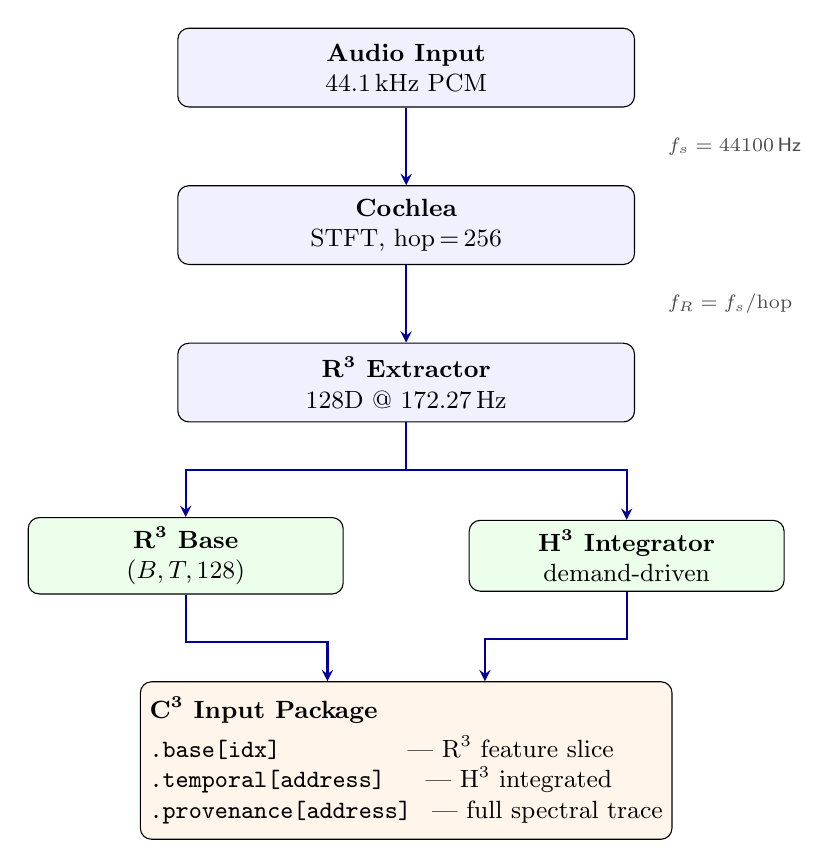
\begin{tikzpicture}[
    block/.style={
        draw, rounded corners=4pt, fill=blue!6,
        minimum width=5.8cm, minimum height=1.0cm,
        font=\small, align=center
    },
    split/.style={
        draw, rounded corners=4pt, fill=green!8,
        minimum width=4.0cm, minimum height=0.9cm,
        font=\small, align=center
    },
    pkg/.style={
        draw, rounded corners=4pt, fill=orange!8,
        minimum width=6.4cm, minimum height=2.0cm,
        font=\small, align=left
    },
    arr/.style={->, >=stealth, thick, color=blue!60!black},
    note/.style={font=\scriptsize\sffamily, color=gray!60!black}
]
    % Top: Audio input
    \node[block] (audio) at (0, 0)
        {\textbf{Audio Input}\\44.1\,kHz PCM};

    % Cochlea
    \node[block] (cochlea) at (0, -2.0)
        {\textbf{Cochlea}\\STFT, hop\,=\,256};
    \draw[arr] (audio) -- (cochlea);
    \node[note, right] at (3.2, -1.0) {$f_s = 44100$\,Hz};

    % R³ Extractor
    \node[block] (r3ext) at (0, -4.0)
        {\textbf{R\textsuperscript{3} Extractor}\\128D @ 172.27\,Hz};
    \draw[arr] (cochlea) -- (r3ext);
    \node[note, right] at (3.2, -3.0) {$f_R = f_s / \mathrm{hop}$};

    % Split into two branches
    \node[split] (r3base) at (-2.8, -6.2)
        {\textbf{R\textsuperscript{3} Base}\\$(B, T, 128)$};
    \node[split] (h3int)  at ( 2.8, -6.2)
        {\textbf{H\textsuperscript{3} Integrator}\\demand-driven};

    \draw[arr] (r3ext.south) -- ++(0,-0.6) -| (r3base.north);
    \draw[arr] (r3ext.south) -- ++(0,-0.6) -| (h3int.north);

    % C³ Input Package
    \node[pkg] (c3pkg) at (0, -8.8)
        {\textbf{C\textsuperscript{3} Input Package}\\[3pt]
         \texttt{.base[idx]}
         \hspace{1.4cm} \textrm{--- R\textsuperscript{3} feature slice}\\
         \texttt{.temporal[address]}
         \hspace{0.3cm} \textrm{--- H\textsuperscript{3} integrated}\\
         \texttt{.provenance[address]}
         \hspace{0.05cm} \textrm{--- full spectral trace}};

    \draw[arr] (r3base.south)  -- ++(0,-0.6) -| ([xshift=-1cm]c3pkg.north);
    \draw[arr] (h3int.south)   -- ++(0,-0.6) -| ([xshift= 1cm]c3pkg.north);
\end{tikzpicture}
\caption{Provenance chain from audio input to C\textsuperscript{3} input package.
         Every tensor element traces back to its R\textsuperscript{3} source
         through spectral addresses.}
\label{fig:provenance}
\end{figure}


%% ============================================================
%%  SECTION 4 — Naming Convention Rules
%% ============================================================
\section{Naming Convention Rules}
\label{sec:naming-rules}

The following rules govern all naming within the Universal Spectral Language.
Violations break the provenance chain and are treated as specification errors.

\begin{enumerate}
    \item \textbf{Measurement, not interpretation.}\enspace
          R\textsuperscript{3} feature names describe what is \emph{measured}
          (e.g.\ \texttt{spectral\_centroid}), never what is
          \emph{perceived} or \emph{interpreted}.

    \item \textbf{No music-theory terms in R\textsuperscript{3}/H\textsuperscript{3}.}\enspace
          Names must not contain \texttt{chord}, \texttt{key},
          \texttt{cadence}, \texttt{tonal}, or \texttt{harmonic}
          in their music-theoretic senses.
          \texttt{harmonic} is permitted only in its signal-processing
          meaning (integer-multiple partials).

    \item \textbf{Perceptual time scales, not musical structure.}\enspace
          H\textsuperscript{3} horizon labels denote perceptual durations.
          For example, \texttt{beat} designates the ${\sim}525$\,ms
          periodicity band, not a musical beat or metrical position.

    \item \textbf{Dot-separated addresses.}\enspace
          Full spectral addresses use dot separation:
          \texttt{feature.horizon.morph.law}.
          No spaces, no slashes, no camelCase.

    \item \textbf{C\textsuperscript{3} music-theory mapping.}\enspace
          C\textsuperscript{3} model documentation \emph{may} reference
          music-theory terms for explanatory purposes, but every such
          reference \emph{must} map to one or more spectral addresses.

    \item \textbf{Unbroken spectral chain.}\enspace
          Every C\textsuperscript{3} input must trace back to an
          R\textsuperscript{3} source through the address system.
          No datum enters C\textsuperscript{3} without a provenance record.
\end{enumerate}
